\documentclass{standalone}
\usepackage{tikz}
\usepackage{ctex,siunitx}
\usepackage{tkz-euclide}
\usepackage{amsmath}
\usetikzlibrary{patterns, calc}
\usetikzlibrary {decorations.pathmorphing, decorations.pathreplacing, decorations.shapes,}
\begin{document}
\small
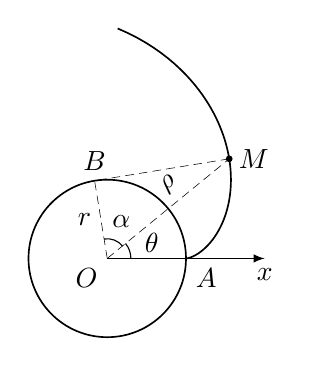
\begin{tikzpicture}[>=latex,scale=1]
  \tkzDefPoints{0/0/O,1/0/A}
  \tkzDefPoint({sqrt(3)/pi*180-60}:{2}){M}
  \draw[thin,->](O)--(2,0)node[below]{$x$};
  \draw [semithick] (0,0)circle(1);
  \draw [semithick,domain=0:70,samples=200] plot ({tan(\x)/pi*180-\x}:{1/cos(\x)});
  \tkzDefLine[tangent from=M](O,A)\tkzGetPoints{B'}{B}
  \tkzDrawSegments[densely dashed](O,B M,B O,M)
  \tkzDrawPoints[fill=black](M)
  \tkzMarkAngle[size=0.25](M,O,B)
  \tkzLabelAngle[pos=0.5](M,O,B){$\alpha$}
  \tkzMarkAngle[size=0.3](A,O,M)
  \tkzLabelAngle[pos=0.6](A,O,M){$\theta$}
  \tkzLabelLine[midway,left,pos=0.5](O,B){$r$}
  \tkzLabelLine[midway,sloped,above,pos=0.6](O,M){$\rho$}
  \tkzLabelPoints[above](B)
  \tkzLabelPoints[below left](O)
  \tkzLabelPoints[below right](A)
  \tkzLabelPoints[right](M)
\end{tikzpicture}
\end{document}